\chapter{Project Architecture} \label{cap:desenvolvimento}

In this chapter, we translate the listed requirements into a selection of specific components to constitute the final system. The primary platform for implementing the artificial intelligence models will be a Raspberry Pi 3B+. The device features 1GB of RAM, which is expected to be sufficient for executing lightweight AI models following preliminary image processing. For prototyping purposes, an OV7670 camera with 300KP resolution (currently owned by a member of the group) may be used; however, if available in the laboratory the final product is intended to utilize a camera with a minimum resolution of 2MP.

\begin{figure}[h!]
    \centering
    \caption{Block diagram with the AIware system architecture}
    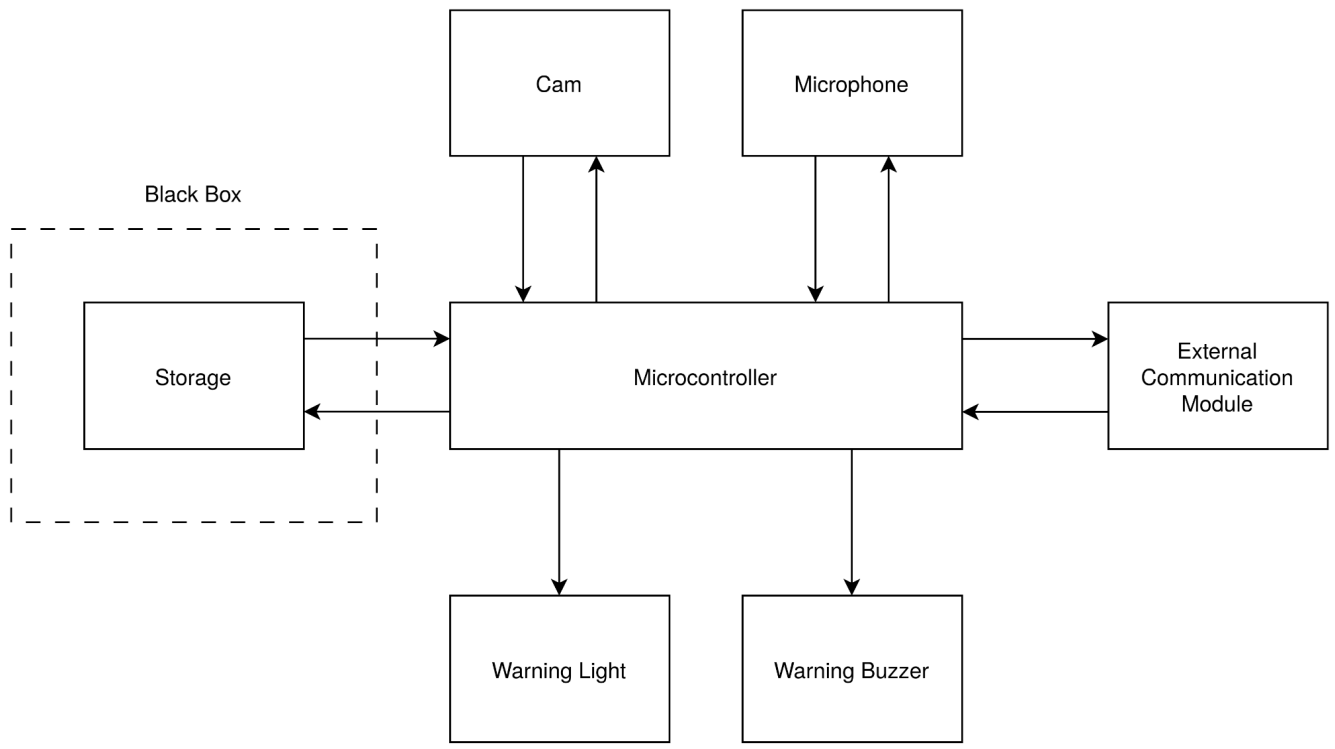
\includegraphics[width=.9\textwidth]{images/architecture.png}
    \label{fig:arch}
\end{figure}

To generate the audible alert, a standard 5V active buzzer will be employed, as it is capable of emitting approximately 85dB at a distance of 10cm, ensuring effectiveness given the system's proximity to the driver. Regarding the visual alert signal, 5mm LEDs are considered for the prototyping phase, with the potential transition to a high-intensity light source for the final version to meet the required luminance specifications.

Regarding external communication, the system implements the MQTT (Message Queuing Telemetry Transport) protocol to transmit driver state and telemetry data to the central monitoring hub. By using MQTT, the AIware system can send periodic updates with minimal protocol overhead, reducing both latency and bandwidth consumption. Furthermore, the protocol's Quality of Service (QoS) levels allow the system to prioritize critical event notifications such as the detection of severe fatigue or a medical emergency ensuring that these alerts are acknowledged by the central server even if the connection is momentarily interrupted.

Initially, LoRa was considered as a possible alternative in our group discussions because of the low volume, low energy consumption and because LoRa stations can cover big distances. However, we opted for MQTT in the end because LoRa requires a dedicated network of gateways. Since a vehicle is mobile and may travel across cities or highways, relying on a provider's private LoRa network is impractical. Using the existing Cellular Network via MQTT seems like a simpler and more straightforward solution.
